\chapter{Opis stworzonego rozwiązania}
\label{cha:rozwiazanie}

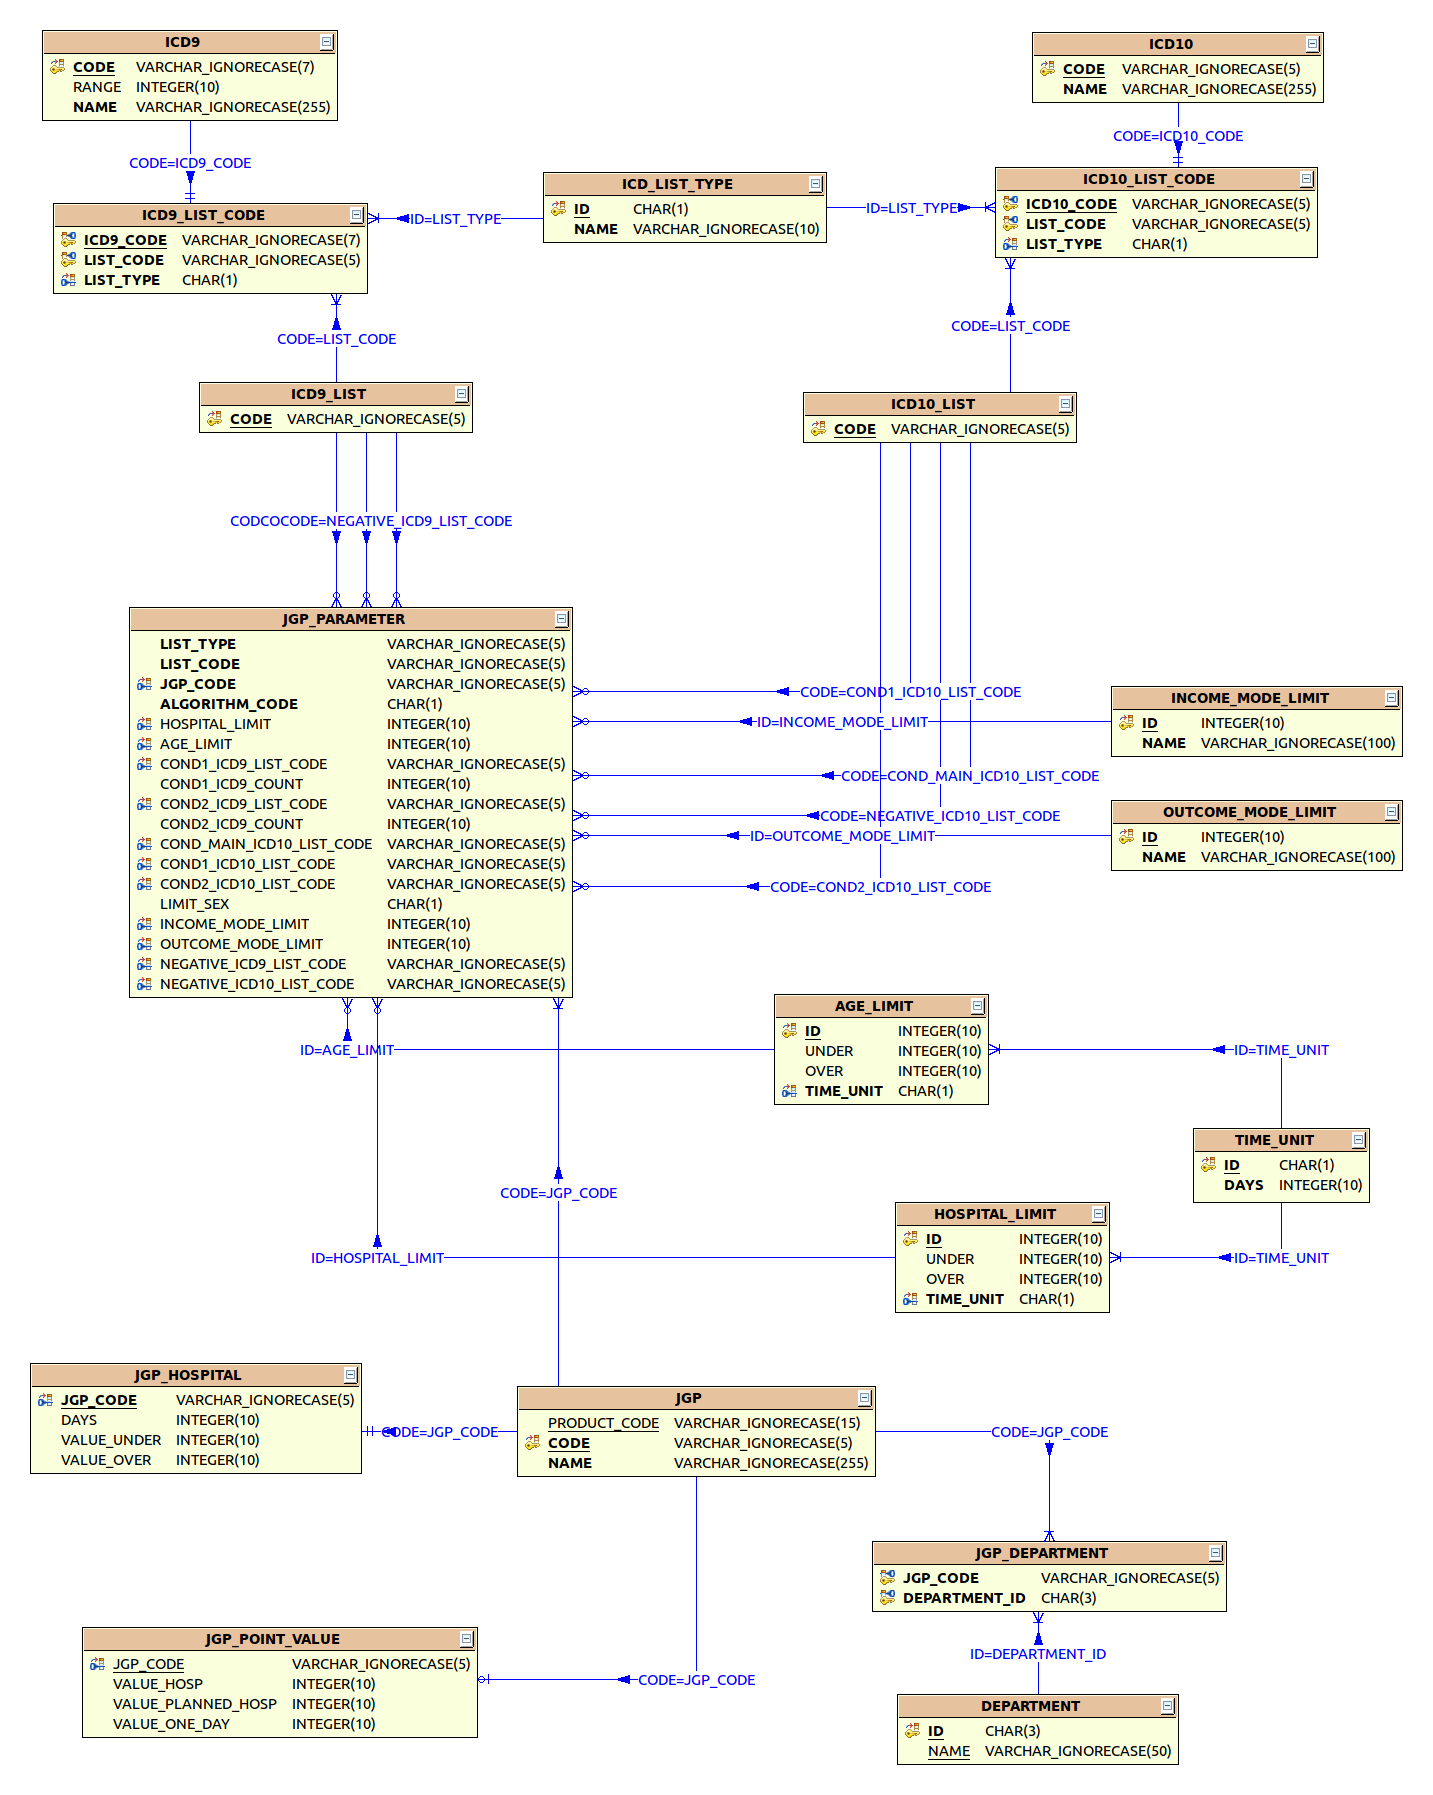
\includegraphics[scale=0.3]{images/erd}

\section{Założenia projektowe}
\label{sec:zalozeniaProjektowe}

\section{Architektura systemu}
\label{sec:architekturaSystemu}

\section{Implementacja}
\label{sec:architekturaSystemu}

\subsection{Konwersja MS-Excel -> relacyjna baza danych}
\label{sec:konwersjaExcelDB}

\subsection{System regułowy w języku JAVA}
\label{sec:systemRegulowyJAVA}

\section{Gruper NFZ}
\label{sec:gruperNFZ}

\subsection{Zasady i logika grupowania}
\label{sec:zasadyLogikaGrupowania}

\subsection{Proces wyznaczania grupy systemu JGP}
\label{sec:procesWyznaczaniaGrupySystemuJGP}

\subsection{Warunki kierunkowe}
\label{sec:warunkiKierunkowe}

\subsection{Mechanizm osobodni}
\label{sec:mechanizmOsobodni}

\section{Optymalizacja JGP}
\label{sec:optymalizacjaJGP}

\subsection{Powody niezaakceptowania do grupy}
\label{sec:powodyNiezaakceptowaniaDoGrupy}
